\documentclass{scrartcl}
\usepackage{authblk}
\usepackage{amsmath}
\usepackage{amssymb}
\usepackage{amsthm}
\usepackage{csquotes}
\usepackage[british]{babel}
\usepackage[
    giveninits,
    backend=biber,
    sorting=none,
    citestyle=numeric-comp,
    maxnames=3,
]{biblatex}
\usepackage{hyperref}
\usepackage{tabularx}
\usepackage{booktabs}
\usepackage{cleveref}
\usepackage{fmtcount}
\usepackage{graphicx}
\DeclareGraphicsExtensions{.pdf}

\usepackage[usenames]{xcolor}
\definecolor{mpl0}{HTML}{1f77b4}
\definecolor{mpl1}{HTML}{ff7f0e}
\definecolor{mpl2}{HTML}{2ca02c}
\definecolor{mpl3}{HTML}{d62728}
\definecolor{mpl4}{HTML}{9467bd}
\definecolor{mpl5}{HTML}{8c564b}
\definecolor{mpl6}{HTML}{e377c2}
\definecolor{mpl7}{HTML}{7f7f7f}
\definecolor{mpl8}{HTML}{bcbd22}
\definecolor{mpl9}{HTML}{17becf}

\hypersetup{
    colorlinks=true,
    linkcolor=mpl0,
    citecolor=mpl0,
    urlcolor=mpl0,
}

\newcommand{\expit}{\sigma}
\newcommand{\transpose}[1]{#1^\intercal}
\newcommand{\observed}[1]{#1}
\DeclareMathOperator{\logit}{logit}
\DeclareMathOperator{\logp}{log1p}
\DeclareMathOperator{\logsumexp}{logsumexp}

\newcommand{\abs}[1]{\left|#1\right|}
\newcommand{\card}[1]{\left|#1\right|}
\newcommand{\population}{N}
\newcommand{\seeds}{U}
\newcommand{\nominees}{V}
\newcommand{\missing}{R}
\newcommand{\blauspace}{\mathbb{B}}
\newcommand{\twocol}[1]{\multicolumn{2}{>{\hsize=\dimexpr2\hsize+3\tabcolsep+2\arrayrulewidth\relax}X}{#1}}

\newcommand{\titlecaption}[2]{\caption[#1]{\emph{#1} #2}}
\newtheorem{prop}{Proposition}
\crefname{prop}{proposition}{propositions}

\newcommand{\tah}[1]{\textbf{[TAH: #1]}}

\addbibresource{main.bib}

% Royal Society Interface Guidance
% Word-count: 2,500 to 8,000 words including cover page, references, and acknowledgements

\title{Inferring social kernels and segregation measures from ego-network data}
\author{Till Hoffmann}
\author{Nick S. Jones}
\affil{Department of Mathematics, Imperial College London}
\date{}

\begin{document}

\maketitle

\begin{abstract} % max 200 words
    How people connect with one another is a fundamental question in the social sciences, and the resulting social networks can have a profound impact on our daily lives. Blau offered a powerful explanation: people connect with one another based on their positions in a social space. Yet a principled measure of social distance in society remains elusive.

    We use the connectivity kernel of conditionally-independent edge models to study distance in Blau space and develop a family of segregation measures with desirable properties: they have an intuitive and universal scale, are applicable to multivariate and mixed node attributes, and capture segregation at the level of individuals, pairs of individuals, and society as a whole. We use the measures to provide visual maps of Blau space---a space spanned by the attributes of the members of society.

    Under a Bayesian paradigm, we infer the parameters of the connectivity kernel from eleven ego network datasets collected in four surveys in the United Kingdom and United States. The importance of different dimensions of Blau space is similar across time and location, suggesting a macroscopically stable social fabric. Physical separation and age differences have the most significant impact on segregation within friendship networks with implications for intergenerational mixing and isolation in later stages of life.
\end{abstract}

\section{Introduction\label{sec:introduction}}

Homophily, the tendency for people to connect with others who are alike, is one of the most robust observations of the social sciences and shapes how our society is connected~\cite{McPherson2001}.
% Whilst institutionalised segregation and discrimination have largely been outlawed in the developed world, voluntary association between individuals who share common traits makes social circles more homogeneous than one would expect by chance.
Quantifying homophily is not only important for understanding why social ties form between some people yet not between others, but the manifestation of homophily as poorly-connected social networks can have a significant impact on dynamics unfolding upon them~\cite{Golub2012}. For example, users of online social networks, such as Facebook and Twitter, tend to connect with others who hold similar political views~\cite{Boutyline2017}. They are more likely to be exposed to information that confirms rather than challenges their beliefs~\cite{Bakshy2015}. An ``echo chamber'' effect ensues, leading to polarised opinions~\cite{DeMarzo2003}. Homophily can also have a detrimental impact on public health: clusters of individuals who mutually reinforce their belief that vaccinations are harmful can raise the likelihood of significant disease outbreaks~\cite{Salathe2008}---even if the vaccination rate is above herd immunity levels on average.

Homophily can be observed in friendships~\cite{Currarini2009, Hipp2009}, networks of discussion partners~\cite{McPherson2006}, communication networks~\cite{Wang2013, Leo2016}, marital ties~\cite{Blau1984}, and online social networks~\cite{Chang2010}. Relationships are homogeneous with respect to a wide range of attributes, including age~\cite{Marsden1988,Smith2014}, gender~\cite{Stehle2011,Smith2014}, ethnicity~\cite{Chang2010, Blumenstock2013, Currarini2009}, education~\cite{McPherson2006, Smith2014,Johnson1989}, occupation~\cite{Chan2004}, income~\cite{Leo2016, Wang2013, Johnson1989}, religion~\cite{Platt2012}, parental~\cite{Johnson1989} and marital status~\cite{Kalmijn2007}, political ideology~\cite{Bakshy2015, Boutyline2017}, and geographical location~\cite{Lambiotte2008, Expert2011, Backstrom2010, Scellato2011, Illenberger2013}. % Romantic relationships, which tend to be heterophilous with respect to gender, are a notable exception.

Segregation measures are often used to quantify homophily~\cite{Rodriguez-Moral2016, Bojanowski2014}. Many approaches are based on co-presence in organisational units such as schools~\cite{Orfield2014}, voluntary associations~\cite{Popielarz1999}, occupations~\cite{Charles1995}, or census tracts~\cite{Reardon2004,Reardon2011}, and we refer to them as \emph{organisational} measures. Typically, they compare how the distribution of demographic attributes within organisational units differs from the distribution of attributes in the general population. Whilst organisational measures are applicable whenever data can be stratified according to a variable of interest, they cannot capture segregation at smaller scales than the strata~\cite{Blumenstock2013}. For example, the ethnic composition of a set of schools may be representative of the general population, indicating that there is no (organisational) segregation. But the social networks \emph{within} schools often exhibit strong ethnic homophily~\cite{Currarini2009,Moody2001}.
%Similarly, social networks exhibit income homophily~\cite{Leo2016}, but neighbourhoods are often heterogeneous with respect to income~\cite{Ioannides2004}.
Organisational measures cannot capture such social segregation.

\emph{Social} measures of segregation, such as the assortativity coefficient~\cite{Newman2003a}, overcome these limitations by explicitly considering the interactions amongst individuals~\cite{Blumenstock2013}, but have their own difficulties: first, they usually rely on the existence of mutually exclusive groups such as sex, ethnicity, or religion~\cite{Bojanowski2014}, and they are not applicable to continuous attributes such as age or income. Attributes are often discretised~\cite{Lam-Morgan2012, Kalmijn2007, Kim2012},
%and models for ``ordered community structure'' in networks have been developed~\cite{Gregory2012},
but the boundaries between categories always suffer from some degree of arbitrariness~\cite{Reardon2004}. Second, segregation for multiple attributes can be measured independently, but it is unclear how to define a composite segregation measure. Furthermore, social measures are typically defined as summary statistics of a fully-observed social network. Consequently, we cannot easily quantify uncertainties. %, and it is non-trivial to apply them to sampled network data.

In practice, the study of homophily is complicated by the scarcity of high-quality data~\cite{Butts2012, Blumenstock2013}: we need social network data together with demographic information for each person. Online social networks and the widespread use of mobile phones provide us with detailed information about connections between individuals~\cite{Golder2014}, and seemingly private traits such as socioeconomic status~\cite{Blumenstock2015, Luo2017}, sexual orientation~\cite{Wang2017}, age, gender, and political ideology can be inferred~\cite{Kosinski2013}. Unfortunately, network features are often used to predict demographic attributes~\cite{Wang2013,Blumenstock2015,Luo2017,Kosinski2013}, which would confound any study of homophily. %: we cannot use the same data to predict demographic attributes and study homophily with respect to those attributes.
Furthermore, data are too revealing in terms of privacy but, at the same time, do not provide enough information for researchers~\cite{Golder2014}. Individuals can be identified in anonymised social networks~\cite{Backstrom2011, Narayanan2008}, and augmenting the network data with demographic information would make re-identification even easier.

However, censuses and large-scale surveys collect comprehensive demographic information from respondents but usually lack data about their associates. Fortunately, some surveys have included questions about respondents' friends~\cite{Huckfeldt1983, Johnson1989}, discussion partners~\cite{Marsden1987, McPherson2006}, or support networks~\cite{Kalmijn2007, Banerjee2013}. The questions used to elicit social ties provide an imperfect observation of the immediate neighbourhood of respondents~\cite{Marin2004,Eagle2015,Eveland-Jr.2017}.

Building on the successes of conditionally-independent edge models~\cite{Snijders2011} and, in particular, latent space models for social networks~\cite{Hoff2002,Handcock2007,Raftery2012}, we consider a generative model for social networks whose members occupy a multidimensional Blau space. We discuss desirable properties for social segregation measures, and, using the generative network model, we develop a suite of measures applicable to arbitrary attributes. The measures capture segregation at different scales: single individuals, pairs of individuals, and society as a whole. We illustrate the measures with a simple example, and we show that it reduces to a well-known segregation measure if the attributes are univariate and categorical.

% In this paper, we aim to address three challenges. First, numerous studies~\cite{Cheadle2012, Currarini2009, Hipp2009,Marsden1987, Marsden1988, McPherson2001, Smith2014, Wimmer2010} refer to Blau's~\cite{Blau1977} intuitive and powerful theory of social structure: people occupy a multidimensional social space spanned by their demographic attributes, and their rates of interaction depend on their relative positions. However, to the best of our knowledge, only \textcite{Hipp2009} explicitly consider such a social space---also referred to as ``Blau space''~\cite{McPherson2001}.

% Second, the difficulties associated with anonymising social network data has sparked interest in generative network models, allowing synthetic data to be shared without risking the privacy of members of the social network~\cite{Pfeiffer-III2014, Lieberman2010, Lieberman2012, Nettleton2016, Sathanur2017}. Yet most investigations of homophily are descriptive and do not consider generative models~\cite{Marsden1981,McPherson2006,Chang2010,Kalmijn2007}.

Furthermore, we derive the posterior for parameters of the conditionally-independent edge model given partial observations of social networks obtained from surveys% and show that the posterior is equivalent to the widely-used ``prior correction'' when the probability for two people to connect is modelled by a logistic model
. We apply our approach to nine existing datasets from the United Kingdom and two from the United States. Our analysis reveals that the effects of homophily on society are remarkably stable in both countries regardless of time and the specific nature of relationships. Using the suite of segregation measures, we find that physical separation and age are the most important factors contributing to the segregation of society. We provide recommendations for conducting surveys to infer homophily in social networks and discuss future work, including principled imputation of demographic attributes in social networks and using the generative model to generate synthetic networks: an approach that has attracted interest to circumvent the difficulties associated with anonymising social network data~\cite{Pfeiffer-III2014, Lieberman2010, Lieberman2012, Nettleton2016, Sathanur2017}.

\section{Methods}

\subsection{Generative network model\label{sec:model}}

% \begin{figure}
%     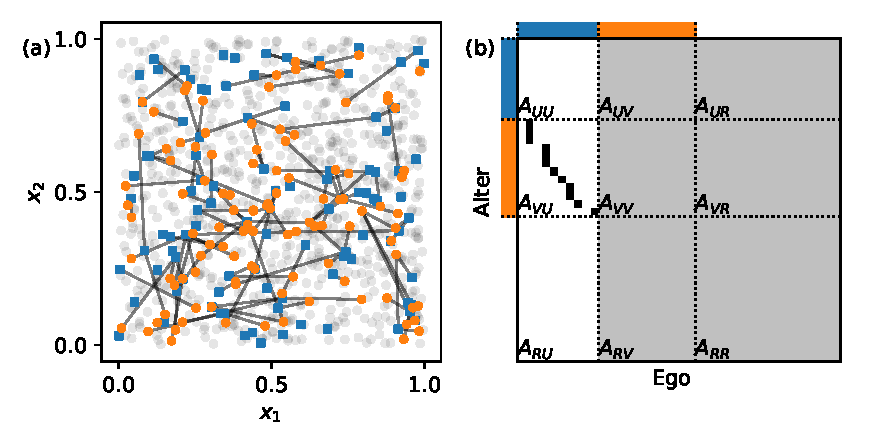
\includegraphics{survey-synthetic}
%     \titlecaption{A simple generative model for ego networks obtained from surveys.}{Panel~(a) shows synthetic survey data generated by our model. Seeds $\seeds$ are represented by blue squares, nominees $\nominees$ by orange circles, and the remainder of the population $\missing$ by grey circles. Panel~(b) illustrates the parts of the adjacency matrix revealed by a particular two-stage survey. Connections are represented by black entries in the adjacency matrix, absent connections by white entries, and lacking information by grey entries.\label{fig:survey-synthetic}}
% \end{figure}

We consider a generative model for social networks for a population of $n$ individuals $\population$ who occupy a Blau space $\blauspace$ spanned by their demographic attributes, such as age, income, or gender. In contrast to common latent space models~\cite{Hoff2002, Hoff2008, Handcock2007}, the attributes are observed, although \textcite{Hoff2002} also consider an extension including covariates. The $q$-dimensional attribute vector $x_i\in\blauspace$ for each individual $i\in \population$ is drawn independently from a distribution $P(x_i)$ of demographic attributes. Elements of the attribute vector can take continuous, ordinal, or categorical values. Connections between individuals are encoded by the binary adjacency matrix $A$ such that $A_{ij}=1$ if $j$ considers $i$ to be a friend and $A_{ij}=0$ otherwise. We assume that people do not interact with themselves such that $A_{ii}=0$ for all $i$, and that connections are undirected, although social ties need not be reciprocated in general~\cite{Ball2013}.

Given the positions of two individuals $i$ and $j$ in Blau space, we assume that connections form independently with probability $\rho(x_i, x_j)$, i.e.\ edges are conditionally-independent given the attributes of nodes~\cite{Fienberg2012}. The assumption of conditionally-in\-de\-pen\-dent edges can be problematic. For example, it is not possible to reproduce heavy-tailed degree distributions if the node density is homogeneous~\cite{Barnett2007}. Furthermore, the average degree scales linearly with the number of nodes unless the connectivity kernel $\rho$ is adjusted to compensate~\cite{Caron2017}. Nevertheless, we use spatial network models because the connectivity kernel is intuitive, and they can capture salient features of social networks. For example, nodes in high-density regions have larger degrees on average~\cite{Barnett2007}. Similarly, members of the ethnic majority have more social ties in social networks in US high schools~\cite{Currarini2009}.

% We now turn to the data collection process. Observations are collected in two stages: first, we sample a subset $\seeds\subset\population$ of \emph{seeds} uniformly at random and collect information about their demographic background. We also ask each seed $j\in \seeds$ about their social ties $\nominees_j=\{i\in\population:A_{ij}=1\}$, henceforth \emph{nominees}. Second, we collect demographic information about the nominees $\nominees=\bigcup_{j\in \seeds} \nominees_j$ by asking the seeds about their friends~\cite{Huckfeldt1983, McPherson2006, Kalmijn2007} or conducting follow-up surveys~\cite{Johnson1989}.

% Panel~(a) of \cref{fig:survey-synthetic} illustrates the model with a simple example: we first draw the positions $x$ of $n=1,000$ nodes in the social space uniformly at random from the two-dimensional unit box. Second, we connect nodes with each another using a connectivity kernel that induces homophily along the two dimensions of Blau space. Finally, we sample $\card{\seeds}=100$ seeds from the population, and collect information about their demographic background as well as their $\card{\nominees}=108$ nominees, which allows us to embed the ego networks in Blau space.

\subsection{Developing a model-based segregation measure}

In addition to addressing the challenges mentioned in \cref{sec:introduction}, a social segregation measure should satisfy the following properties: first, the measure should be insensitive to the overall edge density to facilitate comparison of segregation across different networks. Otherwise, the segregation measure would depend on the size of the population because the edge density scales as $n^{-1}$ if the average degree is approximately constant. Second, following \textcite{Freeman1978}, we would like the measure to capture the notion that segregation places ``restrictions on the access of people to one another''. Third, the measure should be easily interpretable, and it should have a natural notion of the absence of segregation when individuals form connections without regard to their positions in Blau space. For example, the difference of within- and between-group ties considered by \textcite{Krackhardt1988} depends on the sizes of the groups even if there is no homophily: there is no natural reference point.

A single measure cannot capture the complexities of social networks, and we develop a family of measures applicable at different scales: the social separation between any two individuals, the isolation experienced by any one individual, and the social strain experienced by society as a whole. Starting at the microscopic level, we use the generative model to define a measure of \emph{social separation} between two individuals with attributes $x$ and $y$:
\begin{align}
    \varphi(x, y) &= \logit \rho(y,y) - \logit\rho(x,y),\label{eq:social-separation}\\
    \text{where }\logit\rho &= \log\left(\frac{\rho}{1-\rho}\right)\nonumber
\end{align}
are the log odds for a connection to form with probability $\rho$. The probability $\rho(y, y)$ for an individual with attributes $y$ to connect with someone with identical attributes serves as a reference point, and the measure does not depend on the overall edge density. The social separation $\varphi$ may be understood as the isolation experienced by an individual with attributes $x$ as a result of the behaviour of another with attributes $y$. The measure is zero if people do not discriminate with respect to the attributes on which they differ or if two individuals have the same demographic attributes.
% In a heterophilous society, the measure is negative for any pair of individuals.
For a homophilous connectivity kernel, the measure is positive and is a \emph{semi-metric} for Blau space; we will consider a family of connectivity kernels for which $\varphi$ is a true metric in \cref{sec:segregation-distance}.

\begin{prop}\label{prop:segregations-semi-metric}
    If the connectivity kernel is homophilious, symmetric, and the probability $\rho(x,x)$ to connect with others who are alike is independent of $x$, the social separation $\varphi$ is a \emph{semimetric}~\cite{Wilson1931}: it satisfies the properties of a metric, including non-negativity, symmetry, and the identity of indiscernables---except the triangle inequality.
\end{prop}
\begin{proof}
    First, $\varphi(x,y)\geq0$ because homophily implies that $\rho(x, y)<\rho(y, y)$ and $\logit$ is a monotonically increasing function. Second, $\varphi(x,y)=\varphi(y,x)$ because the first term of \cref{eq:social-separation} is constant by assumption and the second is symmetric because the kernel is symmetric. Third, the measure is zero for any two individuals with the same attributes by substitution into \cref{eq:social-separation}. Similarly, if $\varphi(x,y)=0$, then $x=y$ because $\rho(x, y)<\rho(y, y)$.
\end{proof}

The less likely two people are to connect, the larger the social separation between them. The assumptions required for \cref{prop:segregations-semi-metric} to hold may seem restrictive, but they are satisfied by most studies of spatial networks~\cite{Barnett2007,Lambiotte2008,Butts2012,Expert2011}.

Defining social separation in terms of a generative model, i.e.\ using the connectivity kernel rather than a summary statistic of a particular dataset, provides us with two advantages: first, any uncertainty associated with the inferred connectivity kernel naturally propagates to the segregation measure. Second, we can easily consider the properties of the segregation measure under a variety of generative models without having to resort to computationally-expensive Monte Carlo simulations.

For example, consider a stochastic block model (SBM)~\cite{Snijders2011} with $K$ blocks, intra-group connection probability $\rho_\mathrm{same}$, and inter-group connection probability $\rho_\mathrm{different}<\rho_\mathrm{same}$. For two nodes with block membership $x$ and $y$, the social separation is
\begin{equation}
    \varphi(x, y) = \left(1-\delta_{xy}\right)\left(\logit\rho_\mathrm{same}-\logit\rho_\mathrm{different}\right),\label{eq:social-separation-sbm}
\end{equation}
$\delta_{xy}$ is the Kronecker delta. The social separation only depends on block membership, and it is not affected by the size of each block. For members of different blocks, $\varphi$ is the difference of log odds ratios for the existence of intra-group ties as opposed to inter-group ties previously considered by \textcite{Moody2001}.

To quantify segregation at the level of an individual with attributes $x$, we define the \emph{social isolation}
\begin{equation}
    \phi(x) = \int dy \ P(y) \varphi(x, y),\label{eq:segregation-individual}
\end{equation}
which measures the average social separation between an individual with attribute $x$ and members of society whose attribute distribution is $P(y)$. For the SBM, we substitute \cref{eq:social-separation-sbm} into \cref{eq:segregation-individual} and obtain
\begin{equation}
    \phi(x) = (1-P(x))\left(\logit\rho_\mathrm{same}-\logit\rho_\mathrm{different}\right),\label{eq:segregation-individual-sbm}
\end{equation}
where $P(x)$ is the probability to belong to block $x$. Members of all blocks experience the same degree of isolation if the blocks are of the same size. If the sizes are unequal, minorities experience more isolation and majority groups experience less isolation. Indeed, ethnic minorities in schools tend to be more isolated and have fewer social ties~\cite{Currarini2009}.

To understand how segregated society is as a whole, we would like to aggregate the social isoluation $\phi$, but the appropriate statistic depends on the question at hand. For example, if we wanted to study the most isolated subpopulation of society, we should consider $\max_{x\in\blauspace}\phi(x)$. Here, we take a utilitarian approach and, in line with \cref{eq:segregation-individual}, define the \emph{social strain} as
\begin{equation}
    \Phi = \int dx\ P(x) \phi(x),\label{eq:social-strain}
\end{equation}
which quantifies the average social separation amongst members of the society. It is zero when individuals do not discriminate based on attributes, and it can reach arbitrarily large values in a society comprising multiple groups that are completely disconnected. For the SBM, we substitute \cref{eq:segregation-individual-sbm} into \cref{eq:social-strain} and obtain
\begin{align}
    \Phi&= \gamma\left(\logit\rho_\mathrm{same}-\logit\rho_\mathrm{different}\right),\nonumber \\
    \text{where }\gamma&=\sum_{x=1}^K P(x) \left(1 - P(x)\right)\label{eq:segregation-distributional-factor}
\end{align}
is a factor accounting for the relative sizes of the $K$ blocks. The social strain is maximal when the group sizes are equal. If one of the blocks is larger, the strain approaches zero as the sizes of the minority blocks decrease: members of the majority group experiences little social isolation. It is unsurprising that there is no social strain if the society is homogeneous, but the utilitarian approach has a serious limitation: it has little concern for minorities that are not well integrated in society. For equal group sizes, the social strain increases with the number of groups, asymptotically reaching a maximum value of $\logit\rho_\mathrm{same}-\logit\rho_\mathrm{different}$.

\subsection{Distance in Blau space\label{sec:segregation-distance}}

The social separation takes a simple form if the probability for two individuals to connect is a logistic kernel~\cite{Hoff2002}, i.e.\
\begin{equation}
    \logit\rho(x, y, \theta) = \sum_{l=1}^p\theta_l f_l(x,y),\label{eq:logistic-kernel}
\end{equation}
where the $p$-dimensional vector $\theta_l$ parametrises the kernel, and $f(x, y)$ is a set of $p$-dimensional features that are predictive of the connection probability, such as the age difference $f_\text{age}=\abs{x_\mathrm{age}-y_\mathrm{age}}$. The social separation between $x$ and $y$ comprises contributions from the features of the logistic kernel:
\begin{align}
    \varphi(x,y) &= \sum_{l=1}^p\varphi_l(x, y),\label{eq:social-separation-logistic}\\
    \text{where }\varphi_l(x, y) &= \theta_l\left(f_l(y, y) - f_l(x, y)\right)\label{eq:social-separation-contribution}
\end{align}
is the contribution due to a single feature $l$. In fact, $\varphi$ is a true metric for many logistic connectivity kernels.

\begin{prop}
    The social separation $\varphi(x,y)$ is a metric if the kernel is homophilous, i.e.\ $\theta_l<0$, and each feature $f_l(x, y)$ is a constant or a positive affine transform of a metric $d_l(x, y)$, i.e.
    \begin{equation}
        f_l(x, y) = a_l d_l(x, y) + b_l,\label{eq:segregation-feature-affine}
    \end{equation}
    where $a_l > 0$ and $b_l$ are the parameters of the affine transform.
\end{prop}
\begin{proof}
    The social separation $\varphi(x,y)$ is a semi-metric according to \cref{prop:segregations-semi-metric}, and, according to \cref{eq:social-separation-logistic}, it comprises contributions from individual features. Showing that each contribution $\varphi_l(x, y)$ satisfies the triangle inequality is sufficient for $\varphi(x, y)$ to satisfy it, i.e.\ we require
    \begin{equation}
        \varphi_l(x, z) \geq \varphi_l(x, y) + \varphi_l(y, z).\label{eq:segregation-metric-inequality}
    \end{equation}
    Substituting \cref{eq:segregation-feature-affine} into \cref{eq:segregation-metric-inequality} yields
    \begin{equation}
        -\theta_l a_l d_l(x, z)\geq -\theta_l a_l\left[d_l(x, y) + d_l(y, z)\right],\label{eq:segregation-metric}
    \end{equation}
    where we have used the metric property $d_l(x, x) = 0$ for all $x$, and the constant $b_l$ in \cref{eq:segregation-feature-affine} vanishes by \cref{eq:social-separation-contribution}. The inequality in \cref{eq:segregation-metric} holds because $\theta_l<0$ for homophilous kernels, $a_l>0$ by assumption, and $d_l(x, y)$ is a metric. \Cref{eq:segregation-metric-inequality} is trivially satisfied for a constant feature, such as a bias term controlling the overall edge density.
\end{proof}

In other words, the social separation is a true measure of \emph{distance} in the social space with a probabilistic interpretation if features are themselves measures of distance, including all the features we consider subsequently.
% TAH: may have to move that to the application section It remains a true metric for the standardised features we considered in \cref{sec:survey-application} because standardisation is an affine transform.
This observation puts Peter Blau's~\cite{Blau1977} hypothesis that ``the macrostructure of societies can be defined as a multidimensional space of social positions among which people are distributed and which affect their social relations'' on a sound statistical footing: \emph{fitting conditionally-independent edge models allows us to learn the metric of Blau space}. The metric has a universal scale, facilitating comparison across different datasets.

\subsection{Parameter inference given ego network data}

A representative sample of dyads between individuals together with their demographic attributes is not generally available. However, a number of surveys have collected information about the social ties of respondents using name-generator questions which elicit social ties by asking respondents to nominate their friends~\cite{Kalmijn2007}, individuals they feel close to~\cite{Hipp2009}, or discussion partners~\cite{Marsden1987,McPherson2006}. To generate examples of disconnected dyads, we consider a random sample of pairs of individuals. To account for this non-ignorable data collection process, we introduce a variable $I_{ij}\in\{0,1\}$ indicating whether a particular dyad $A_{ij}$ was observed. The available data thus comprise the demographic attributes $x$ of individuals included in the sample and the dyad state $A_{ij}$ (1 if $i$ and $j$ are connected and $0$ otherwise) if it was observed, i.e.\ $I_{ij}=1$. Adapting the argument presented by \textcite{King2001} to a Bayesian paradigm, we consider the posterior distribution over kernel parameters $\theta$ given the available data:
\begin{equation}
    P(\theta|\observed{A}, \observed{f}, I=1)\propto P(\observed{A}|\theta,\observed{f},I=1)P(\theta),\label{eq:parameter-posterior}
\end{equation}
where $P(\theta)$ is the kernel parameter prior, and $f=f(x,y)$ are features sufficient to evaluate the connectivity kernel given demographic attributes $x$ and $y$.
%$\observed{A}=\left\{A_{ij} : I_{ij} = 1\right\}$ denotes the set of all observed dyads,
The observed-data likelihood is
\begin{equation}
    P(\observed{A}|\theta,\observed{f},I=1)=\frac{P(\observed{f}|\observed{A},\theta,I=1)P(\observed{A}|\theta,I=1)}{P(\observed{f}|\theta,I=1)}.\label{eq:observed-likelihood}
\end{equation}
Considering the first term in the numerator of \cref{eq:observed-likelihood}, we note that the distribution over kernel features given the state $A$ of the dyad does not depend on whether it was included in the sample or not. More formally,
\begin{align}
    P(f|A,\theta,I=1)&=P(f|A,\theta)\\
    &=\frac{P(A|f,\theta)P(f|\theta)}{P(A|\theta)}.\label{eq:conditional-equivalence}
\end{align}
Turning to the denominator in \cref{eq:observed-likelihood}, we find
\begin{align}
    P(f|\theta,I=1)&=\sum_{\alpha=0}^1 P(f|A=\alpha,\theta,I=1)P(A=\alpha|\theta,I=1)\nonumber\\
    &=P(f|\theta)\sum_{\alpha=0}^1 P(A=\alpha|f,\theta)\frac{P(A=\alpha|\theta,I=1)}{P(A=\alpha|\theta)},\label{eq:likelihood-denominator}
\end{align}
where we used the identity in \cref{eq:conditional-equivalence} to arrive at the second line. Substituting \cref{eq:conditional-equivalence,eq:likelihood-denominator} into \cref{eq:observed-likelihood}, the observed-data likelihood is
\begin{align}
    P(A|\theta,f,I=1)&=\frac{P(A|f,\theta)r(A)}{\sum_{\alpha=0}^1 P(A=\alpha|f,\theta)r(\alpha)},\label{eq:observed-likelihood-final}\\
    \text{where }r(\alpha)&=\frac{P(A=\alpha|\theta,I=1)}{P(A=\alpha|\theta)}\nonumber
\end{align}
is the ratio of prevalences of dyad state $\alpha$ in the sample and the general population. In practice, we approximate the prevalence ratio $r$ using the empirical sample prevalence and prior knowledge about the prevalence in the population. The posterior can be evaluated by substituting \cref{eq:observed-likelihood-final} into \cref{eq:parameter-posterior}, and we can thus infer the parameters $\theta$ from ego network data. See \cref{app:numeric-stability} for details on how to evaluate the observed-data log-likelihood in a numerically stable fashion.

\section{Application}

\subsection{Ego network data collected in surveys\label{sec:application}}

The social ties identified through name-generator questions depend on the nature of the relationship, the mode of administration of the questionnaire (e.g.\ face-to-face, telephone interview, or online survey), and the interviewer~\cite{Marin2004,Eagle2015}. Consequently, we do not expect the kernel parameters inferred from different datasets to be completely consistent. In the following investigation of ego networks, we restrict the nature of relationships to friends who are not relatives as much as the available data permit: we are interested in \emph{voluntary} association amongst members of the population rather than the social structures they were born into~\cite{Kalmijn2007}.

Demographic information about nominees can be collected either by asking seeds about their friends' demographic background~\cite{Marsden1987,McPherson2006} or by conducting follow-up surveys~\cite{Johnson1989}. The latter seems preferable because respondents may not have complete information about their social contacts, but the approach requires additional resources to interview the nominees and may suffer from low response rates. For example, the age of nominees in the British Household Panel Survey (BHPS), one of the datasets we consider, is 60\% more likely to be an integer multiple of ten than it is for seeds---presumably because seeds round the age of their friends to the nearest decade. In anticipation of such challenges, the coding for the nominees is often coarser than for seeds. To compare the demographic attributes of seeds and nominees we need to unify the coding (see \cref{app:coding-and-features} for details for each dataset).

% Second, the number of terms contributing to the sum in \cref{eq:survey-weighted-log-likelihood} becomes prohibitively large as the number of observed dyads grows---especially when evaluated repeatedly by a Metropolis-Hastings sampler. We use a random subset of seed pairs to evaluate the log likelihood. In fact, the number of controls does not have a significant impact on the inference as long as the number is sufficiently large, as discussed in \cref{prop:survey-bias-correction,prop:survey-asymptotic-hessian}.

\subsection{General Social Survey\label{sec:survey-gss}}

The General Social Survey (GSS) is a nationally-representative face-to-face survey of non-institutionalised adults living in the US. Demographic attributes of seeds are collected regularly and include age, sex, ethnicity, religion, and education~\cite{Marsden1987,Marsden1988}. In 2004, respondents were asked about the demographic background of people ``with whom they discuss important matters'', which tends to elicit close ties~\cite{Marin2004}. We omit all nominees who are not considered to be friends or who are family. The coding of age and sex is consistent amongst seeds and nominees. We aggregate the detailed coding of ethnic and religious attributes of seeds to match the coding of nominees, as shown in \cref{tbl:survey-gss-coding}. Kernel features include the absolute age and ordinal education level difference as well as binary indicators for differences along the sex, ethnicity, and religion dimensions.

Some of the demographic attributes of seeds and nominees are missing because respondents did not know or refused to provide the information, and we drop dyads associated with individuals with one or more missing attributes, as shown in \cref{tbl:survey-sample-size}. Such a complete-case analysis can introduce biases if the data are not missing completely at random~\cite{Rubin1976}, but handling the missing data in a principled fashion would require us to develop a model for demographic attributes~\cite{Pigott2001, Gelman2013}.

For each demographic attribute, we define a feature for the logistic kernel in \cref{eq:logistic-kernel}, as shown in \cref{tbl:survey-gss-coding}. To standardise the features $f(x_i,x_j)$, we subtract their mean and divide non-binary features by twice their standard deviation~\cite{Gelman2008a}; binary features are not rescaled. The statistics are calculated with respect to a random sample of pairs of seeds. Feature standardisation allows us to compare kernel parameters more easily~\cite{Gelman2008a} and simplifies the formulation of priors: we use independent, weakly-informative Cauchy priors for the kernel parameters such that
\[
    P(\theta_l) \propto {\left[1+{\left(\frac{\theta_l}{\alpha_l}\right)}^2\right]}^{-1}.
\]
Following \textcite{Gelman2008}, we chose the scale parameters $\alpha_l=2.5$ for $l>1$ to represent our weak prior belief that changing a feature by one standard deviation is unlikely to change the log odds by more than five: the independent Cauchy distributions regularise the kernel parameters by placing significant prior probability near zero, but their heavy tails allow for significant departures from zero should the data be in support of large parameters. % Specifying the scale parameters would have been more cumbersome without feature standardisation. For example, different scale parameters need to be chosen for the parameter controlling age homophily depending on whether age is recorded in months, years or decades.
We set $\alpha_1=10$ because the parameter $\theta_1$ associated with the constant bias term could change significantly depending on the population size~\cite[chapter 16]{Gelman2013}.

\begin{figure}
    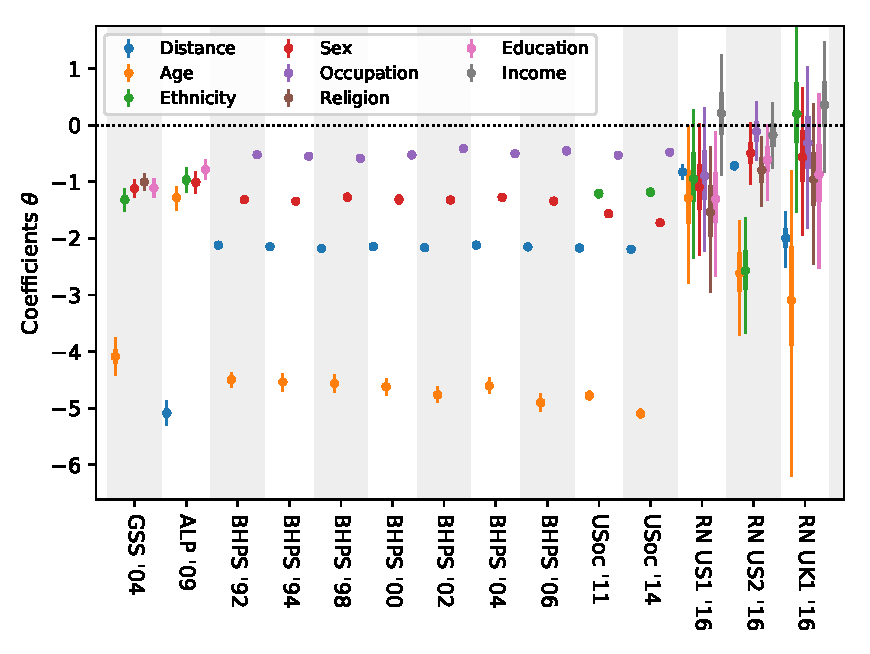
\includegraphics[width=.6\columnwidth]{survey-coefficients}
    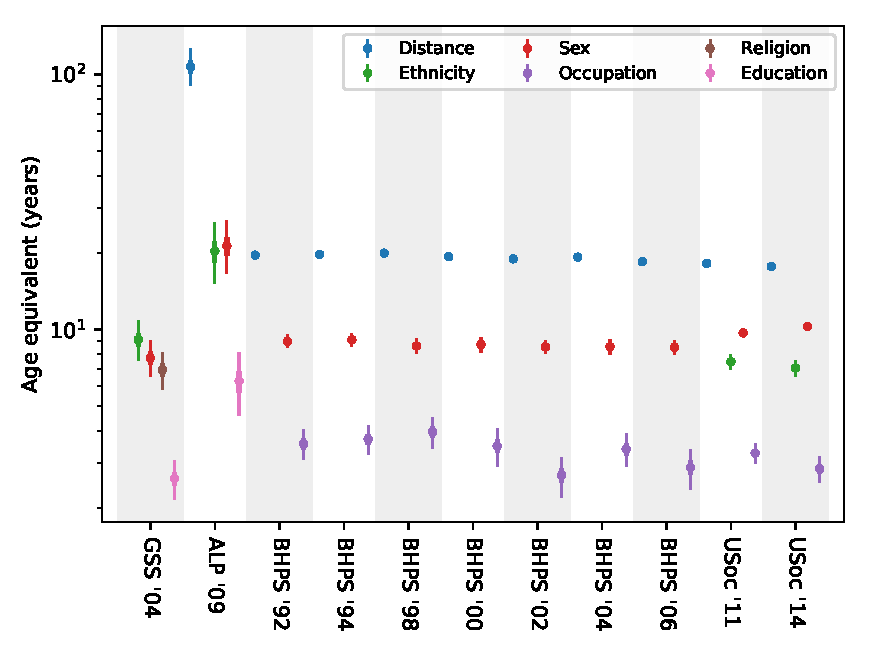
\includegraphics[width=.6\columnwidth]{survey-age-equivalent}
    \tah{need to update figures}
    \titlecaption{Age and physical separation have a strong impact on connection probabilities, and converting parameters into age equivalents makes feature comparison more intuitive.}{
    Panel~(a) shows kernel parameters inferred from ego network data for each dataset.
    Panel~(b) shows age equivalents. For binary features (sex, occupation, religion, ethnicity, and distance for the American Life Panel), the equivalent number of years corresponds to a change from having the same attribute to having a different attribute. Age equivalents for the American Life Panel are overestimated (see \cref{sec:survey-alp} for details).
    Markers represent the posterior mean, thick error bars the interquartile range, and thin error bars the 95\% posterior interval.\label{fig:parameters-and-age-equivalents}}
\end{figure}

The inference is performed in two steps: first, we maximise the posterior with respect to the parameters $\theta$ using a gradient ascent algorithm. Second, we run a Metropolis-Hastings algorithm to draw samples from the posterior~\cite{Hastings1970}. Summary statistics of the posterior are shown in \cref{fig:parameters-and-age-equivalents}~(a). The connection probabilities decrease quickly with increasing age differences. Ethnic, sex, educational, and religious differences all seem to have a similar effect and decrease the odds of connection by a factor of about 0.4 each.\tah{double check numbers}

\textcite{Hipp2009} used the logarithm of physical separation as a benchmark to translate the effect of other attributes into distance-equivalents. We instead use age as a benchmark because age is available for most datasets and is typically coded uniformly in years. In contrast, physical separation is often not available or coded heterogeneously across different datasets. For example, the American Life Panel only provides location information at the state level (see \cref{sec:survey-alp}), whilst the British Household Panel Survey recorded distance between seeds and nominees as ordinal data (see \cref{sec:survey-bhps-usoc}). For the GSS, being of a different ethnicity is equivalent to a nine-year age difference, and having a different sex or religion translates to eight and seven years, respectively. One educational level, as defined in \cref{tbl:survey-gss-coding}, corresponds to three years, as shown in \cref{fig:parameters-and-age-equivalents}~(b).

\subsection{American Life Panel\label{sec:survey-alp}}

The American Life Panel (ALP) is a nationally-representative panel of adults resident in the US.\@ Panel members are interviewed either using their own internet connection or are provided with a web television to access surveys. Data are collected regularly and each survey has a different focus. In 2009, information about social networks and financial literacy was collected. Demographic attributes included sex, age, ethnicity, education, their state of residence, and whether respondents identified as Hispanic. Respondents were also asked to nominate others with whom they ``discuss financial matters''~\cite{Mihaly2009}. We only include nominees who are friends of seeds and exclude kinship ties; see \cref{tbl:survey-alp-coding} for details of harmonisation of attributes across seeds and nominees.

Homophily with respect to sex, ethnicity, and education is slightly weaker but not inconsistent with the GSS.\@ Age differences appear to play less of a role in the discussion of financial matters at first sight, but the inference is severely biased for age. We cannot resolve strong age homophily because data are only recorded in 15-year bins: the small age parameter is likely a result of regression dilution caused by measuring ages imprecisely~\cite{Hutcheon2010}. Consequently, the age equivalents in \cref{fig:parameters-and-age-equivalents}~(b) are inflated. Being resident in a different state has by far the most significant impact on friendship formation.

\subsection{British Household Panel Survey and Understanding Society\label{sec:survey-bhps-usoc}}

The British Household Panel Survey (BHPS) was a nationally-representative face-to-face survey in the UK.\@ It was conducted from 1991 to 2008 and has since been replaced by the Understanding Society (USoc) survey. Respondents were asked questions about ``their closest friends'' every other year as part of the BHPS and every three years in USoc. Data include sex, age, occupational status, ethnicity (only in USoc), and how far away friends live~\cite{Institute-for-Social-and-Economic-Research2000,Institute-for-Social-and-Economic-Research2017} (see \cref{tbl:survey-usoc-coding} for details).

% \begin{figure}
%     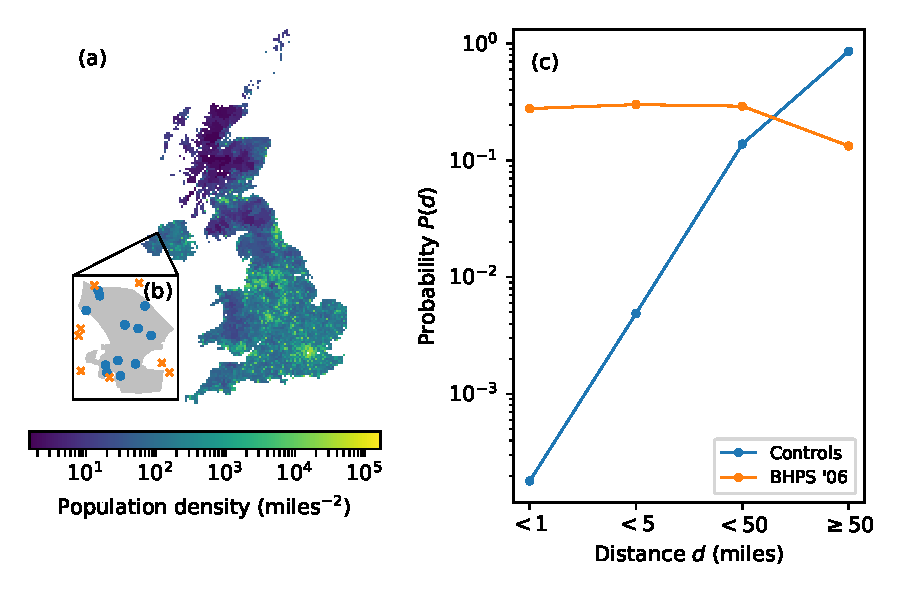
\includegraphics{survey-distances}
%     \titlecaption{We obtain the distribution of distances between people using Monte Carlo sampling.}{Panel~(a) shows the population density in the UK derived from lower layer super output areas. Panel~(b) illustrates the sampling method for home locations using rejection sampling. The reference distribution of distances between randomly chosen home locations and the distribution of distances between seeds and nominees is shown in panel~(c).\label{fig:survey-distances}}
% \end{figure}

The inferred kernel parameters are largely consistent with the inference for the ALP and GSS in the US suggesting that friendship formation proceeds similarly in the two countries. We have omitted data from the BHPS in 2008 because we identified errors in the coding which have since been confirmed by the Institute of Social and Economic Research~\cite{Hoffmann2016}. Similarly, we omitted data from the BHPS in 1996 because physical separation between friends was not recorded. As shown in \cref{fig:parameters-and-age-equivalents}, homophily with respect to sex seems to have increased in recent years but it is unclear whether this observation is the result of people forming friendships differently or a different data collection process~\cite{Hoffmann2017}.

\subsection{Inferred segregation}

\begin{figure}
    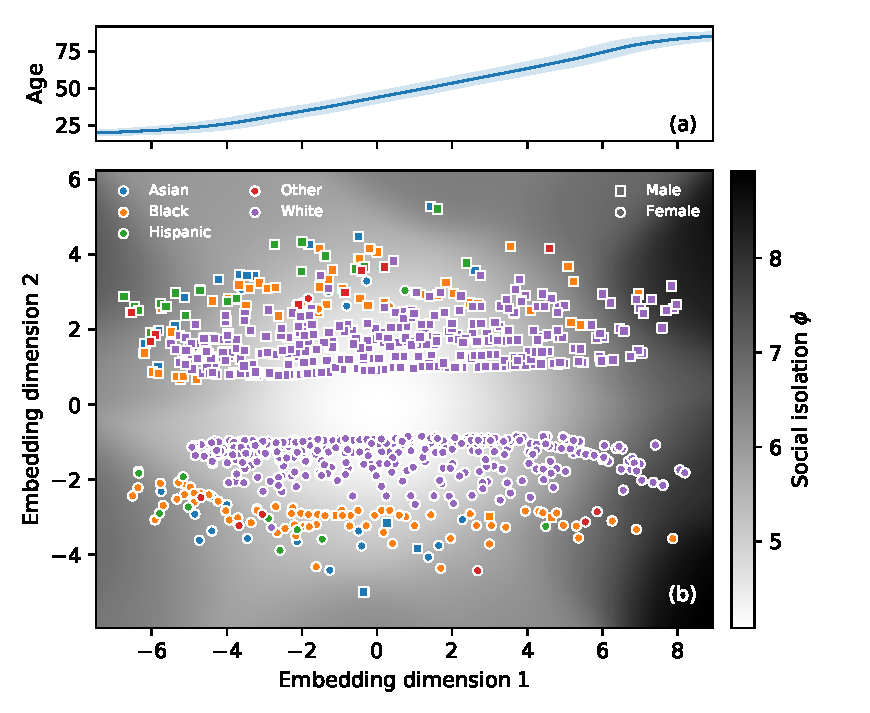
\includegraphics{segregation-embedding}
    \titlecaption{A lower-dimensional embedding of the inter-node distances reveals an interpretable social space.}{Panel~(a) shows the mean and standard deviation of ages as a function of the first embedding dimension as a solid line and a shaded region, respectively. Panel~(b) shows a scatter plot of respondents in a two-dimensional embedding space whose coordinates were obtained from the social separation $\varphi$ using multidimensional scaling. The colour of a marker indicates the respondent's ethnicity and the shape indicates their sex. The heat map represents a smoothed estimate of the social isolation $\phi$.\label{fig:segregation-embedding}}
\end{figure}

To get a better understanding of Blau space and the metric induced by the connectivity kernel, we consider a sample $S$ of 1,000 respondents from the General Social Survey and compute the social separation between them to obtain a distance matrix
\[
    \hat\varphi_{ij} = \transpose{\hat\theta}\left(f(x_j, x_j)-f(x_i, x_j)\right),
\]
where $\hat\theta$ is the posterior mean of the kernel parameters discussed in \cref{sec:survey-gss}. We use multidimensional scaling to embed the respondents in a two-dimensional space~\cite{Borg1996}, as shown in \cref{fig:segregation-embedding}. Panel~(b) shows the two-dimensional embedding that best approximates the distance matrix in the high-dimensional social space. Some men (squares) can be found amongst the cluster of women (circles) and vice versa because the optimisation algorithm converged to a local minimum.

The first dimension captures the age of respondents, as illustrated in panel~(a): the mean age increases monotonically as a function of the first embedding dimension, and the standard deviation is small. We evaluated both statistics using Gaussian kernel smoothing~\cite[chapter~6]{Hastie2009}. The second dimension captures sex and ethnicity. As expected from \cref{eq:segregation-individual-sbm}, ethnic minorities are more isolated and live on the outskirts of society while the ethnic majority occupies the centre. The embedding suggests that age has the strongest impact on how people form friendships.

Panel~(b) of \cref{fig:segregation-embedding} also shows the social isolation $\phi$ experienced by individuals as a greyscale heat map which we obtained in two steps: first, we evaluated an estimate of the social isolation
\[
    \hat\phi_i = \frac{1}{\card{S}-1}\sum_{j\in S:j\neq i} \hat\varphi_{ij}.
\]
Second, we applied Gaussian kernel smoothing to the social isolation in the embedding space. Respondents occupying the centre of society experience little isolation whereas individuals in the periphery are more isolated.

\begin{figure}
    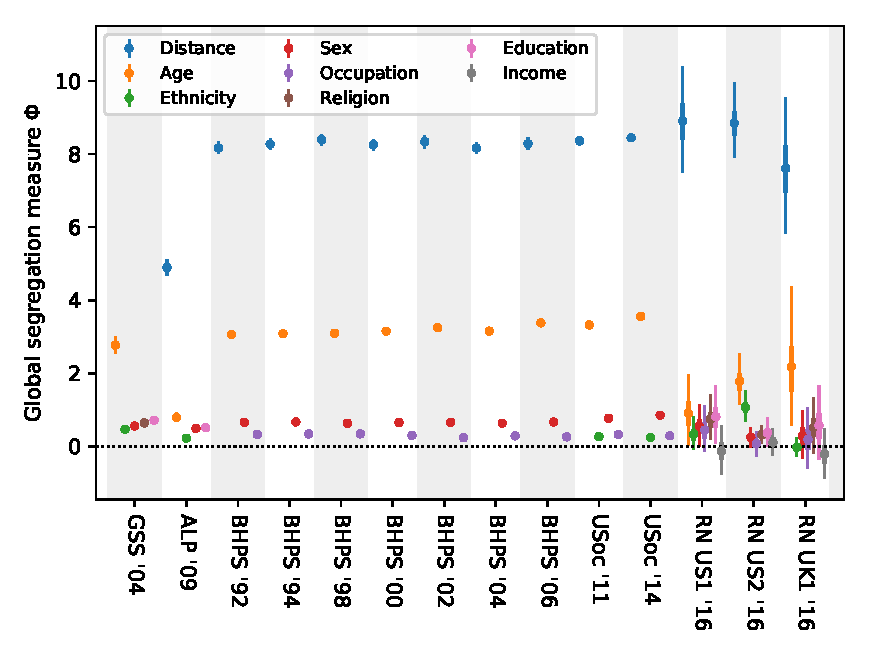
\includegraphics{segregation-survey}
    \titlecaption{Physical separation and age differences are the most important factors preventing integration of society for all datasets.}{Markers represent the posterior mean of the contributions to social strain for each feature, thick error bars the interquartile range, and thin error bars the 95\% posterior interval.\label{fig:segregation-survey}}
\end{figure}

Similar to the social separation in \cref{eq:social-separation-logistic}, the social strain can be broken down into components
\begin{equation}
    \Phi_l = \theta_l \int dx\ dy\ \left(f_l(y, y) - f_l(x, y)\right)\label{eq:segregation-contributions}
\end{equation}
because it is a linear functional of $\varphi$: each component contributes to the social strain in society. For each of the datasets, we evaluate an estimate of the contributions to the social strain
\[
    \hat\Phi_l = \frac{2\hat\theta_l}{\card{\seeds}(\card{\seeds}-1)} \sum_{i < j\in\seeds:i\neq j} \left[f_l(x_j, x_j)-f_l(x_i, x_j)\right],
\]
where the sum is over all distinct pairs of seeds $\seeds$. The contribution $\Phi_l$ measures the average social separation due to feature $l$, and it captures the effect of both the connectivity kernel $\rho(x,y)$ and the attribute distribution $P(x)$: neither is sufficient on its own to quantify segregation. Furthermore, $\Phi$ and its contributions in \cref{eq:segregation-contributions} have an intuitive interpretation and universal scale, facilitating comparison across different datasets. In contrast, whilst standardising the features makes the comparison of kernel parameters easier~\cite{Gelman2008a}, correlations amongst the features and skewed feature distributions can make them misleading~\cite{Greenland1986}. For example, physical space has by far the most significant impact on how members of society connect with one another, as shown in \cref{fig:segregation-survey}. The consistent, large contribution to the social strain due to spatial effects in the BHPS, USoc survey, and ALP survey are at odds with the varying magnitude of kernel parameters we inferred in \cref{sec:survey-gss,sec:survey-alp,sec:survey-bhps-usoc}. A possible explanation for the difference between kernel parameters and the social strain is that individuals adjust their preferences based on the local population density~\cite{Backstrom2010}. In other words, the number of ``intervening opportunities''~\cite{Stouffer1940,Illenberger2013} for making connections may be more important than the physical distance such that individuals in low-density areas are less discriminative and form longer-range ties~\cite{Liben-Nowell2005}.

The importance of physical space highlights that our suite of segregation measures does not distinguish between \emph{choice homophily} and \emph{opportunistic homophily}~\cite{Franz2010}. The former is a result of individuals having an active preference to connect with others who are alike, whereas the latter is a result of individuals being exposed to others who are similar to them. For example, residents of a neighbourhood that is largely homogeneous with respect to ethnicity may not have an active preference for connecting with others of the same ethnicity, but most friendships are likely to be homogeneous because there are fewer opportunities to connect with others of a different ethnicity. Opportunistic homophily is likely to be a large contributing factor to spatial homophily because individuals are less likely to encounter people who live far from them.

Age homophily places the second strongest restriction on how people connect with one another, and it is more than three times as restrictive as any other feature except physical space. The ALP survey is an exception because of the regression dilution~\cite{Hutcheon2010} discussed in \cref{sec:survey-alp}. Age homophily is known to be particularly strong for friendship networks~\cite{McPherson2001}.

Homophily with respect to sex, ethnicity, education, religion, and occupation make similar, small contributions to the segregation of society. Importantly, the social strain captures the average contribution to social isolation: it can be small either because there is little homophily or because there is a large majority group, as evident from~\cref{eq:segregation-distributional-factor}. For example, almost 80\% of respondents in the GSS identify as ``White'' and experience little social isolation due to their ethnicity, whereas minority groups experience more social isolation. On average, social isolation due to ethnicity is small.

\section{Discussion}

We considered a generative model for social networks embedded in Blau space, a space spanned by the demographic attributes of members of society. Investigating social distance in Blau space, we developed a family of segregation measures with a universal scale, facilitating comparison between datasets collected at different times or in different cultural contexts. Furthermore, the segregation measures are applicable to mixed attribute types, have a natural reference point, and an intuitive interpretation. Based on eleven ego network datasets collected in the United Kingdom and United States, we inferred the connectivity kernel $\rho(x,y)$, i.e.\ the probability for an individual with demographic attributes $x$ to connect with another with attributes $y$. Using the kernel, we compared segregation across different datasets along different demographic dimensions and found that physical distance and age have the most significant impact on how well society is connected.

Even though we did not expect the kernel parameters to be consistent across countries, time, or even different surveys, people connected with one another in a surprisingly similar fashion across the different datasets (the BHPS and USoc are longitudinal studies such that consistent parameter estimates are less surprising). Our observations, together with a study by \textcite{Mossong2008} finding that ``mixing patterns [\ldots] were remarkably similar across different European countries'', suggest that a universal connectivity kernel for friendships may exist. To test this hypothesis, further surveys should be conducted in a unified fashion to minimise the effects of question wording and how the survey is administered~\cite{Eagle2015}. In particular, such surveys should explore options to explicitly incentivise nominees to provide data about themselves~\cite{Biernacki1981}: seeds may not recall certain attributes, or nominees may deliberately portray themselves inaccurately~\cite{Bruch2016}. Questions regarding ethnicity should allow respondents to provide multiple answers such that people with mixed ethnic backgrounds can express their identity. Rather than asking respondents about potentially sensitive information, such as income, proxy information that is more readily available---and potentially more informative of how individuals interact with society---could be collected~\cite{Po2012}. Whenever possible, aggregation of attributes such as age into bins should be avoided because it limits the ability to infer kernel parameters~\cite{Hutcheon2010}, as we saw in \cref{sec:survey-alp}.

% We dropped individuals with incomplete demographic attributes from our analysis which may have biased the kernel parameters~\cite{Rubin1976}. % We expect any potential bias to be small because the number of dropped individuals is small~\cite{Pigott2001}.
% More sophisticated approaches such as model-based imputation may improve the inference~\cite{Pigott2001}.

The connectivity kernel is an intuitive model of how people connect with one another, and it is able to reproduce some of the statistics of real social networks. For example, people in high-density regions of Blau space have been observed to have more connections~\cite{Currarini2009}. However, exponential random graph models may be able to better capture the nature of social networks~\cite{Wimmer2010}. Furthermore, we have used a connectivity kernel that: (a)~is symmetric and cannot identify whether there is a status order in society~\cite{Chan2004,Ball2013}, and (b)~only depends on differences between individuals. For example, young men tend to have more social contacts than young women, and older women have more social contacts than older men~\cite{Bhattacharya2016}---an observation that cannot be captured by a kernel of the form we have considered. The connectivity kernel could be refined by adding the demographic attributes of the seeds and nominees as features, capturing sociability and popularity, respectively. Furthermore, it should be determined whether the number of ``intervening opportunities''~\cite{Stouffer1940}, absolute distance in Blau space, or a hybrid thereof are most predictive of tie probability. Ultimately, learning a connectivity kernel without a pre-specified parametric form should be considered~\cite{Frolich2006}. But interpretable summary statistics, such as the family of segregation measures we considered here, are useful for comparisons across societies even for non-parametric kernels.

Because our approach is based on a generative model of social networks, it can generate synthetic social networks which can be studied without privacy risks~\cite{Nettleton2016}. Similarly, the model can be used to impute missing attributes of individuals in social networks. In contrast to other methods, which generally only produce point estimates~\cite{Wang2013, Backstrom2010}, our approach yields a posterior distribution over demographic attributes that captures uncertainties.

For certain logistic connectivity kernels, the social separation is a metric for Blau space and allows us to quantify social distance in a principled fashion. We used the metric to evaluate the social distance amongst respondents to the GSS.\@ Using a lower-dimensional embedding of the respondents, we explored Blau space, corroborating our findings that age has a profound impact on restricting friendship formation.

Whilst the social strain is able to summarise segregation at the level of an entire society, it is not suitable for studying the isolation experienced by minority groups because of its utilitarian foundations. Future work should consider other summary statistics of the social separation and isolation measures in the context of particular social questions. For example, using equal weights for different ethnicities in \cref{eq:social-strain}, rather than weighting by their prevalence in the general population, would yield a measure that does not disadvantage minority groups. Unfortunately, equal weighting does not easily generalise for continuous attributes and further efforts are required.

\printbibliography

\appendix
\numberwithin{equation}{section}
\numberwithin{figure}{section}
\numberwithin{table}{section}

\section{Evaluation of the observed-data log-likelihood}

\subsection{Weighting to account for non-uniform inclusion probabilities}

Seeds are often not included in the survey uniformly at random, and weights are traditionally used to compensate for the potentially biased selection of respondents~\cite{Kish1992}. Including weights in Bayesian analyses is generally difficult~\cite{Gelman2007}, and, in principle, we should model the data collection process explicitly~\cite[chapter~8]{Gelman2013}. Unfortunately, modelling the data collection process is non-trivial, and we use a weighted pseudo-likelihood instead~\cite{Pfeffermann1996}. In particular, the observed-data log-likelihood from \cref{eq:observed-likelihood-final} becomes
\begin{multline}
    L = \sum_{(i,j):I_{ij} = 1} w_j\left\{A_{ij} + (1 - A_{ij})w_i\right\}
    \\\times\left\{A_{ij}\log\rho_{ij} + (1-A_{ij})\log(1-\rho_{ij})-\log\left[r(0)(1 - \rho_{ij}) + r(1)\rho_{ij}\right]\right\},\label{eq:survey-weighted-log-likelihood}
\end{multline}
where $w_j$ is the weight associated with seed $j$. We clip all weights exceeding the \ordinalnum{95} percentile of the empirical weight distribution and normalise them such that $\sum_{j\in\seeds}w_j=\card{\seeds}$. Censoring the weights, also known as Winsorisation, limits the variance induced by attributing variable importance to different observations at the expense of introducing a small bias~\cite{Kish1992}.

\subsection{Numerical stability\label{app:numeric-stability}}

The evaluation of the observed-data log-likelihood may suffer from numerical instabilities, especially when the connectivity kernel is small. We can mitigate such instabilities for logistic connectiviy kernels, i.e.
\begin{align}
    \rho(x,y,\theta)&=\expit(\transpose{\theta}f(x,y)),\\
    \text{where }\expit(\xi)&=\frac{1}{1+\exp(-\xi)}
\end{align}
is the logistic function. In particular, note that $1 - \expit(\xi) = \expit(-\xi)$ and $\log\expit(\xi)=-\logp\exp(-\xi)$, where $\logp(\xi)=\log(1 + \xi)$ is a numerically stable implementation---even for $\abs{\xi}\ll 1$. Substituting into \cref{eq:observed-likelihood-final} yields
\begin{multline}
    \log P(A|f,\theta,I=1)= -\sum_{(i,j):I_{ij}=1} A_{ij}\logp\exp\left(-\transpose{\theta}f_{ij}\right)+\left(1-A_{ij}\right)\logp\exp\left(\transpose{\theta}f_{ij}\right) \\
    + \logsumexp\left[\log r(0) - \logp\exp\left(\transpose{\theta}f_{ij}\right) + ,\log r(1)-\logp\exp\left(-\transpose{\theta}f_{ij}\right)\right],
\end{multline}
where $\logsumexp(x_1, \ldots, x_k)=\log\sum_{i=1}^k\exp(x_k)$ is a numerically stable implementation.

\section{Coding of demographic attributes and feature maps\label{app:coding-and-features}}

In the BHPS and USoc surveys, distance was coded as an ordinal variable: less than one mile, less than five miles, less than fifty miles, and more than fifty miles. We rely on having complete information about seeds to evaluate the control features in \cref{eq:logistic-kernel}. But data on the residential location of seeds is not made available to protect their privacy. Fortunately, we can sample the home locations of respondents\footnote{Sampling home locations cannot reproduce any correlation between home location and other demographic attributes.} using population estimates and the geographic boundaries of lower layer super output areas (LSOAs). LSOAs are census reporting areas and have a few thousand inhabitants each~\cite{Lsoas}. We approximate the distribution of distances between residents of the UK using rejection sampling:
%, as illustrated in \cref{fig:survey-distances}:
first, choose a LSOA with probability proportional to the number of residents. Second, choose one of the polygons associated with the LSOA with probability proportional to the area of the polygon (LSOAs are not necessarily contiguous). Third, sample points uniformly inside the bounding box of the polygon until a point inside the polygon is sampled. The last two steps assume uniform population densities within each LSOA, which is unlikely to be problematic as they are small areas. Having sampled the residential location of two respondents, we calculate the distance between respondents and cast to the same ordinal scale as reported for nominees. USoc furthermore distinguishes between friends living more than fifty miles apart but within the UK and friends outside the UK. We discard the latter (3.6\% and 2.8\% of all friends in waves C and F of USoc) because it is difficult to define an appropriate control population. For the BHPS, we implicitly assume that all friends are resident in the UK.

In USoc, respondents could identify with mixed ethnicities, and we coded such responses as a mixed membership. For example, a respondent who indicated ``mixed Asian and White'' would belong to both White and Asian ethnicities. To measure how different two people are in terms of ethnicity, we define the feature map
\[
    f_\text{ethnicity}(x_i, x_j) = \frac{1}{2} \sum_{l\in E}\abs{x_{il}-x_{jl}},
\]
where $E$ is the set of attributes encoding ethnic identity, and ethnicity memberships are normalised such that $\sum_{l\in E}x_{jl}=1$ for all $j$. For example, $f_\text{ethnicity}(x_i, x_j)=1$ for two people $i$ and $j$ one of which identifies as white and the other as black. For a person $i$ identifying as black and another person $j$ identifying as mixed black and Asian, $f_\text{ethnicity}(x_i, x_j)=0.5$.

\begin{table}
    \begin{tabularx}{\columnwidth}{lXXc}
        \toprule % =================================================================================
        Variable & Seed coding & Nominee coding & $f(x, y)$ \\
        \midrule % ---------------------------------------------------------------------------------
        Bias term &\twocol{\dotfill}& $1$\\
        Age & \twocol{Age in years\dotfill} & $\left|x-y\right|$\\
        Sex & \twocol{(a)~Male, (b)~Female\dotfill} & $x\neq y$\\
        Ethnicity & (a)~\{Asian Indian, Chinese, Filipino, Japanese, Korean, Vietnamese, Other Asian\} (b)~Black, (c)~Hispanic, (d)~White, (e)~\{American Indian or Alaska Native, Native Hawaiian, Guamanian or Chamorro, Samoan, Other Pacific Islander, Other\}& (a)~Asian, (b)~Black, (c)~Hispanic, (d)~White, (e)~Other & $x \neq y$\\
        Religion & (a)~Protestant, (b)~Catholic, (c)~Jewish, (d)~None, (e)~\{Other, Buddhism, Hinduism, Islam, Orthodox, Christian, Native American, Nondenominational\} & (a)~Protestant, (b)~Catholic, (c)~Jewish, (d)~None, (e)~Other & $x\neq y$ \\
        Education & (1)~1--6 years, (2)~7--12 years without high school diploma, (3) exactly 12 years with high school diploma, (4) $>12$ years without degree, (5)~Associate degree, (6)~Bachelor's degree, (7)~Professional or graduate degree & (1)~1--6 years, (2)~7--12 years, (3)~High school graduate, (4)~Some college, (5)~Associate degree, (6)~Bachelor's degree, (7)~Professional or graduate degree & $\left|x-y\right|$\\
        \bottomrule % ==============================================================================
    \end{tabularx}
    \titlecaption{Coding of the demographic variables for the General Social Survey together with the feature maps for each variable.}{Seeds were provided with 16 options to choose from for their own ethnicity but only five options for their nominees. We attempt to unify the educational coding by combining the number of years of education and formal qualifications of the seeds to approximate the coding of nominees. The bias term in the first row of the table controls the overall edge density.\label{tbl:survey-gss-coding}}
\end{table}

\begin{table}
    \begin{tabularx}{\columnwidth}{lrrrr}
        \toprule % =================================================================================
        Dataset & Seeds & Dropped seeds & Nominees & Dropped nominees \\
        \midrule % ---------------------------------------------------------------------------------
        GSS 2004        & 2,785     & 27 (1.0\%) & 869 & 164 (15.9\%) \\
        ALP 2009        & 2,511     & 0 (0.0\%) & 895 & 171 (16.0\%) \\
        BHPS 1992       & 9,427     & 32 (0.3\%) & 19,126 & 601 (3.0\%) \\
        BHPS 1994       & 9,019     & 38 (0.4\%) & 17,609 & 481 (2.7\%) \\
        BHPS 1998       & 8,864     & 30 (0.3\%) & 17,309 & 459 (2.6\%) \\
        BHPS 2000       & 8,603     & 23 (0.3\%) & 16,742 & 441 (2.6\%) \\
        BHPS 2002       & 8,277     & 18 (0.2\%) & 16,276 & 496 (3.0\%) \\
        BHPS 2004       & 7,937     & 31 (0.4\%) & 15,430 & 455 (2.9\%) \\
        BHPS 2006       & 7,785     & 19 (0.2\%) & 14,836 & 383 (2.5\%) \\
        USoc 2011       & 37,718    & 505 (1.3\%) & 77,163 & 1,062 (1.4\%) \\
        USoc 2014       & 30,163    & 325 (1.1\%) & 64,630 & 829 (1.3\%) \\
        % RN US1 2016     & 848       & 186 (18.0\%) & 19 & 3 (13.6\%) \\
        % RN US2 2016     & 1,811     & 177 (8.9\%) & 79 & 20 (20.2\%) \\
        % RN UK1 2016     & 864       & 148 (14.6\%) & 10 & 2 (16.7\%) \\
        \bottomrule % ==============================================================================
    \end{tabularx}
    \titlecaption{Number of retained seeds and nominees for each dataset together with the number of individuals who have been excluded from the analysis because one or more of their demographic attributes were missing.}{\label{tbl:survey-sample-size}}
\end{table}

\begin{table}
    \begin{tabularx}{\columnwidth}{lXXc}
        \toprule % =================================================================================
        Variable & Seed coding & Nominee coding & $f(x, y)$ \\
        \midrule % ---------------------------------------------------------------------------------
        Bias term &\twocol{\dotfill}& $1$\\
        Age & Age in years recoded to match the nominee coding & Age brackets in years: (1)~0--20, (2)~21--35, (3)~36--50, (4)~51--65, (5)~66--80, (6)~$>80$ & $\left|x-y\right|$\\
        Sex & \twocol{(a)~Male, (b)~Female\dotfill} & $x\neq y$\\
        Ethnicity & \twocol{(a)~White or Caucasian, (b)~Black or African American, (c)~American Indian or Alaska Native, (d)~Asian or Pacific Islander, (e)~Hispanic (see below) (f)~Other} & $x \neq y$\\
        Hispanic & \twocol{(a)~Yes, (b)~No; ethnicity is coded as ``Hispanic'' if response is affirmative.\dotfill} & \\
        Education & \twocol{The seed coding is more refined but can be reduced to the nominee coding: (1)~Less than \ordinalnum{9} grade, (2)~\ordinalnum{9}--\ordinalnum{12} grade without diploma, (3)~High school graduate, (4)~Some college, (5)~Associate degree, (6)~Bachelor's degree, (7)~Master's degree, (8)~Professional degree or doctorate\dotfill} & $\left|x-y\right|$\\
        State & \twocol{One of 52 states and Washington DC and Puerto Rico\dotfill} & $x \neq y$\\
        \bottomrule % ==============================================================================
    \end{tabularx}
    \titlecaption{Coding of the demographic variables for the American Life Panel together with the feature maps for each variable.}{We aggregate the ages and educational attainments of seeds to match the coarser coding of nominees, as shown in \cref{tbl:survey-alp-coding}. The joint effect of ethnic differences and whether people identify as Hispanic is still unclear~\cite{Smith2017a}; for consistency with the GSS, we code the ethnicity of respondents as ``Hispanic'' if they consider themselves to be Hispanic or Latino irrespective of their reported ethnicity. In fact, 46\% of respondents who identified as Hispanic selected ``other'' as their ethnicity, compared with $<1\%$ for respondents who did not identify as Hispanic.\label{tbl:survey-alp-coding}}
\end{table}

\begin{table}
    \noindent\begin{minipage}{\columnwidth}
    \renewcommand*\footnoterule{}
    \begin{tabularx}{\columnwidth}{lXXc}
        \toprule % =================================================================================
        Variable & Seed coding & Nominee coding & $f(x, y)$ \\
        \midrule % ---------------------------------------------------------------------------------
        Bias term &\twocol{\dotfill}& $1$\\
        Age & \twocol{Age in years\dotfill} & $\left|x-y\right|$\\
        Sex & \twocol{(a)~Male, (b)~Female\dotfill} & $x\neq y$\\
        Occupation & (a)~\{Self-employed, employed, maternity leave, unpaid worker in family business\footnote{\label{ft:survey-only-usoc}Only available in Understanding Society.}\}, (b)~\{Unemployed, disabled\}, (c)~\{Full-time student, government training scheme\}, (d)~Family care, (e)~Retired & (a)~\{Full-time employed, part-time employed\}, (b)~Unemployed, (c)~Full-time education, (d)~Full-time housework, (e)~Retired & $x \neq y$\\
        Distance & Only applicable to the seed-nominee pair & (1)~$<1~\mathrm{mile}$, (2)~$<5~\mathrm{miles}$, (3)~$<50~\mathrm{miles}$, (4)~$\geq50~\mathrm{miles}$ but still in the UK &\footnote{We use the ordinal distance measure reported in the survey as a regression feature and generate control features using Monte Carlo simulation, as discussed in \cref{sec:survey-bhps-usoc}.}\\
        Ethnicity\footref{ft:survey-only-usoc} & \twocol{Independent binary choices: White, Asian, Black, Other\dotfill} &\footnote{See \cref{sec:survey-bhps-usoc} for a detailed description of the feature map.}\\
        \bottomrule % ==============================================================================
    \end{tabularx}
    \end{minipage}
    \titlecaption{Coding of the demographic variables for the British Household Panel Survey and Understanding Society together with the feature maps for each variable.}{Sex and age have identical coding for seeds and nominees. We aggregate the detailed occupational coding of seeds to match the coding of nominees. In particular, we code women on maternity leave as employed because their occupational status is only temporary, and we code disabled individuals as ``not employed'' because they are unlikely to have the same social opportunities as people in employment.\label{tbl:survey-usoc-coding}}
\end{table}

\end{document}
